Para que você se prepare adequadamente para o seu TCC, além de ler este manual e conhecer as regras e práticas adotadas no NUCOMP, nós sugerimos algumas leituras essenciais.

\noindent\begin{minipage}{0.8\textwidth}
\textbf{Título}. Metodologia de Pesquisa Em Ciência da Computação\\
\textbf{Autor}. Raul Wazlawick\\
\textbf{Editora}. Campus Elsevier\\
\textbf{Ano}. 2014\\
\end{minipage}\begin{minipage}{0.2\textwidth}
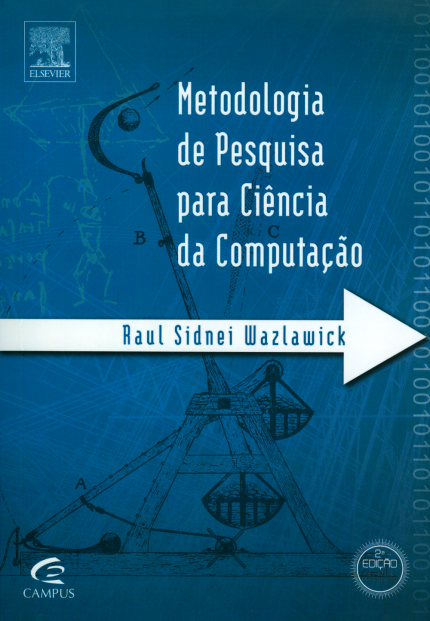
\includegraphics[width=\linewidth]{./img/wazlawick}
\end{minipage}

\noindent \begin{minipage}{0.8\textwidth}
\textbf{Título}. Guia Prático para Redação Científica\\
\textbf{Autor}. Gilson Volpato\\
\textbf{Editora}. Best Writing\\
\textbf{Ano}. 2015\\
\end{minipage}\begin{minipage}{0.2\textwidth}
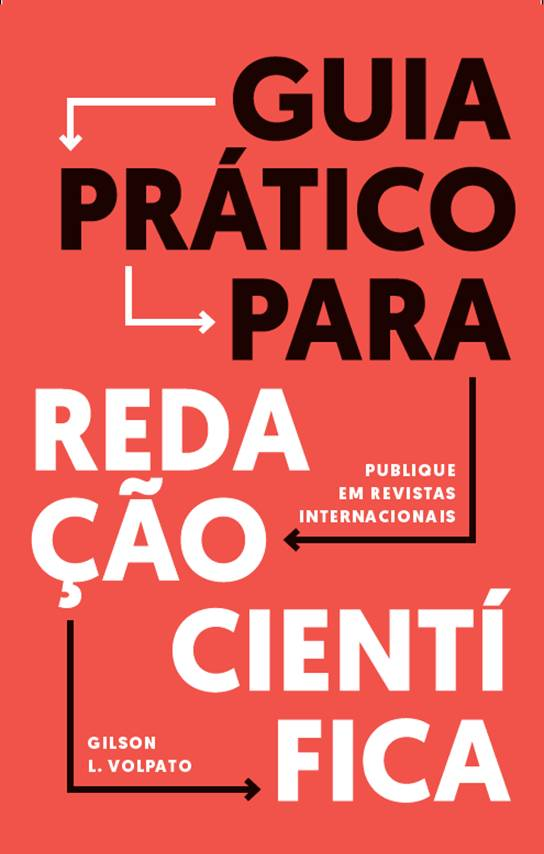
\includegraphics[width=\linewidth]{./img/volpato}
\end{minipage}

\noindent \begin{minipage}{0.8\textwidth}
\textbf{Título}. Elaboração de Projeto, TCC, Dissertação e Tese \\
\textbf{Autor}. Mario de Souza Almeida\\
\textbf{Editora}. Atlas\\
\textbf{Ano}. 2014\\
\end{minipage}\begin{minipage}{0.2\textwidth}
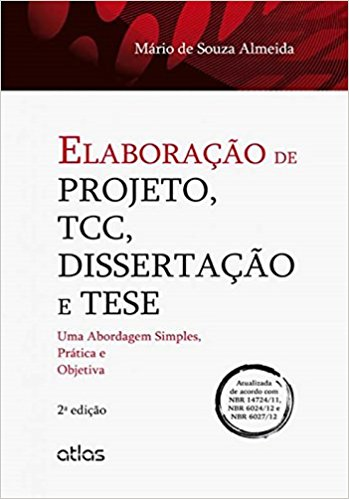
\includegraphics[width=\linewidth]{./img/almeida}
\end{minipage}
